% Preamble
% Document type
\documentclass{article}

% Additional packages
\usepackage[utf8]{inputenc}

% Clickable Links in TOC
\usepackage[hidelinks]{hyperref}

% Images/ figures package
\usepackage{graphicx}
\graphicspath{ {./images/} }

% Language
\usepackage[ngerman]{babel}

% Information
\title{Projekt DeskPlanner}
\author{Pinar Gökcek, Kyle Mezger, Jay Imort, Rico Hofmann, Darios Pachtsinis}
\date{04. April 2022}

% Content
% Beginning of document
\begin{document}

% Titlepage
\begin{titlepage}
    \centering
    % Output title
    \maketitle

    % Fill rest of page
    \vfill

\end{titlepage}

% Table of contents
\tableofcontents

\pagebreak

\section{Zielgruppe, Problem, Eigenschaften, Alleinstellungsmerkmal}

\subsection{Zielgruppe}

\subsection{Problem}
Problemstellung:

Während der Pandemiezeit wird verstärkt von Zuhause aus gearbeitet, dadurch schwankt die Anzahl der Arbeiter im Büro stark und die interdisziplinären Kollegen habe keinen Überblick mehr darüber, wer im Büro ist und wer nicht. Zumal grundsätzlich nicht jeder in das Home-Office kann bzw. will, dies kann diverse Gründe, wie z. B. fehlende Räumlichkeiten oder die geschwächte Konzentrationsfähigkeit in den eigenen vier Wänden sein. Agile Arbeitsplätze haben den Vorteil, dass der Arbeitsplatz je nach momentanem empfinden gewählt werden kann z. B. im sogenannten Ruhebereich, Bereiche die näher an Heizkörpern sind oder hellere Arbeitsplätze an Fenstern. Projektspezifisch kann es vorteilhaft sein neben einem bestimmten Kollegen zu arbeiten, um den Austausch produktiver zu gestalten. Diese Bereiche können frei benutzt werden, sofern diese nicht durch eine andere Kollegin oder einen anderen Kollegen belegt sind. Derzeit ist es gängig, dass die Bereiche nach dem Prinzip “first come first serve“ besetzt werden.\\\\
Wenn man am Morgen an einem Arbeitsplatz sitzt, dann aber im Laufe des Tages für einen längeren Zeitraum diesen verlassen muss, wird diese Ressource unnötig blockiert. Raumbelüftungssysteme, Heizungen und Klimaanlagen für Räume bzw. Gebäude werden nicht nach der Personenauslastung betrieben, in Hinblick auf die steigenden Energiekosten, ist dies weder ökonomisch noch nachhaltig.
Immungeschwächte Personen die ihre Tätigkeit nur vor Ort im Büro erledigen können, haben pandemiebedingt nicht die Möglichkeit Arbeitsplätze zu Buchen, die weiter weg von den restlichen Arbeitsplätzen bzw. Kollegen sind. Der Arbeitgeber, der nur eine bestimmte X Arbeitsplätzen hat, kann nicht mehr als X Arbeiter in dem Bürokomplex beschäftigen. Desweitern gibt es derzeit keine einfache Möglichkeit die Büro Belegschaft, über einen längeren Zeitraum zu analysieren. Diese Analyse kann unter anderem zur dauerhaften Arbeitsplatz Reduktion, bei gleicher Mitarbeiterzahl führen.\\\\
Unsere Anwendung ermöglicht es, die oben angesprochenen Fälle zu Gunsten des Arbeitgebers und -nehmers zu lösen.  Die Raumplanung ermöglichet eine Buchung in 15 min Rastern auch Dauerbuchungen über mehrere Monate sind möglich. Nicht nur Arbeitsplätze in einem Raum, sondern bestimmte Räume in bestimmten Gebäuden können gebucht werden. Auch ist eine Chatfunktion zwischen Teamleitern und Mitarbeitern bzw. zwischen Mitarbeitern möglich. Dies hat den Vorteil das Buchungen bei Sonderfällen unter Mitarbeitern einfach getauscht werden können. Eine Synchronisation mit dem Outlookkalender wäre auch denkbar.

\subsection{Eigenschaften}
Die Web-Applikation DeskPlanner wird mindestens folgende Eigenschaften nachweisen können:

\begin{itemize}
    \item Open Source (Lizenzfrei) als kostenfreie Möglichkeit für vor allem kleine Unternehmen
    \item Simple Möglichkeiten, um Komplexität zu vermeiden, aber so viele Möglichkeiten der Raumplanung beizubehalten
    \item Three-Tier Architecture ähnliche Anwendungsweise der Raumplanung im Sinne von Gebäude > Stockwerk > Raum 
\end{itemize}

Des Weiteren sind kleine Eigenschaften wie Einhaltung der 7 Usability Prinzipien vorgesehen, um so die Bedienung des Kunden so einfach wie möglich zu halten. 
Beispiele hierfür sind Hilfstexte, welche die verschiedenen Buttons erklären sollen oder selbsterklärende Icons der jeweiligen Buttons. 
Außerdem soll der Nutzer nicht mit Information beschüttet werden, sondern eine auf seinen Nutzungskontext angepasste Benutzeroberfläche sorgen für Aufgabenangemessenheit. 
Durch die individuelle Raumgestaltung erhält der Nutzer ein steuerbares Softwaresystem, welches genau das machen wird, was der Nutzer auch erwartet.

\subsection{Alleinstellungsmerkmal}
Als herausragendes Leistungsmerkmal des DeskPlanners bezeichnet man die effiziente Arbeitsplatznutzung. 
In der heutigen Branche, vor allem durch Corona bestätigt, gilt es, die Kosten immer weiter zu reduzieren. 
Durch die Raumbuchungsmöglichkeiten, kann ein Unternehmen die Arbeitsplätze minimieren, Home Office Mitarbeiter perfekt einplanen und dadurch Kosten der Technik und Größe des Raumes einsparen für andere Investitionen. 
Als Open Source Web-Applikation kann ein Unternehmen sogar lizenzfrei den Arbeitsplatz kosteneffizienter nutzen.
Genau hier soll der DeskPlanner vor allem kleineren Unternehmen unterstützen, um auch in Zeiten der Pandemie nicht insolvent zu gehen.
\pagebreak
\section{User Stories}

Mitarbeiter/-in:

\begin{itemize}
    \item Als Mitarbeiter/-in möchte ich Sitzplätze anschauen, damit ich in einem Blick sehe welche Plätze verfügbar/vergeben sind.

    \item Als Mitarbeiter/-in möchte ich Sitzplätze buchen, damit ich für die gebuchte Zeit einen Arbeitsplatz zur verfügung habe.

    \item Als Mitarbeiter/-in möchte ich Sitzplätze abonnieren, damit ich einen Sitzplatz über längere Zeit zu einer gewissen Zeit reserviert habe ohne jeden Tag einzeln buchen zu müssen.

    \item Als Mitarbeiter/-in möchte ich Sitzplätze stornieren, damit ich bei einer Fehlbuchung oder Krankheit den Platz für andere Mitarbeiter wieder buchbar machen kann.

    \item Als Mitarbeiter/-in möchte ich mit einem Platz Besitzer chatten können, damit ich anfragen kann ob der jeweilige Platz verfügbar gemacht werden könnte.

    \item Als Mitarbeiter/-in möchte ich Nachrichten erhalten, damit ich bei der Anfrage eines anderen Mitarbeiters meinen gebuchten Platz für diesen stornieren kann.
\end{itemize}

\noindent Admin:

\begin{itemize}
    \item Als Administrator/-in möchte ich alle Funktionen des Mitarbeiters haben, da ich mitunter Mitarbeiter bin.

    \item Als Administrator/-in möchte ich das Layout von Räumen anpassen, damit es dem tatsächlichen Büro entspricht und es somit besser erkennbar ist für Mitarbeiter um welchen Raum und Sitzplatz es sich handelt.

    \item Als Administrator/-in möchte ich Gruppen verwalten können, damit ich Bestimmte Positionen und Personen in Gruppen einteilen kann, damit ein Geschäftsführer diese in Raumbuchungen beschränken kann.
\end{itemize}

\noindent Geschäftsführer/-in:

\begin{itemize}
    \item Als Geschäftsführer/-in möchte ich alle Funktionen des Mitarbeiters haben, da ich mitunter Mitarbeiter bin.

    \item Als Geschäftsführer/-in möchte ich die Buchbarkeit von Räumen auf Gruppen einschränken, damit bestimmte Räume für bestimmte Positionen/Personen ausgelegt sind.
\end{itemize}
\begin{figure}[h]
    \centering
    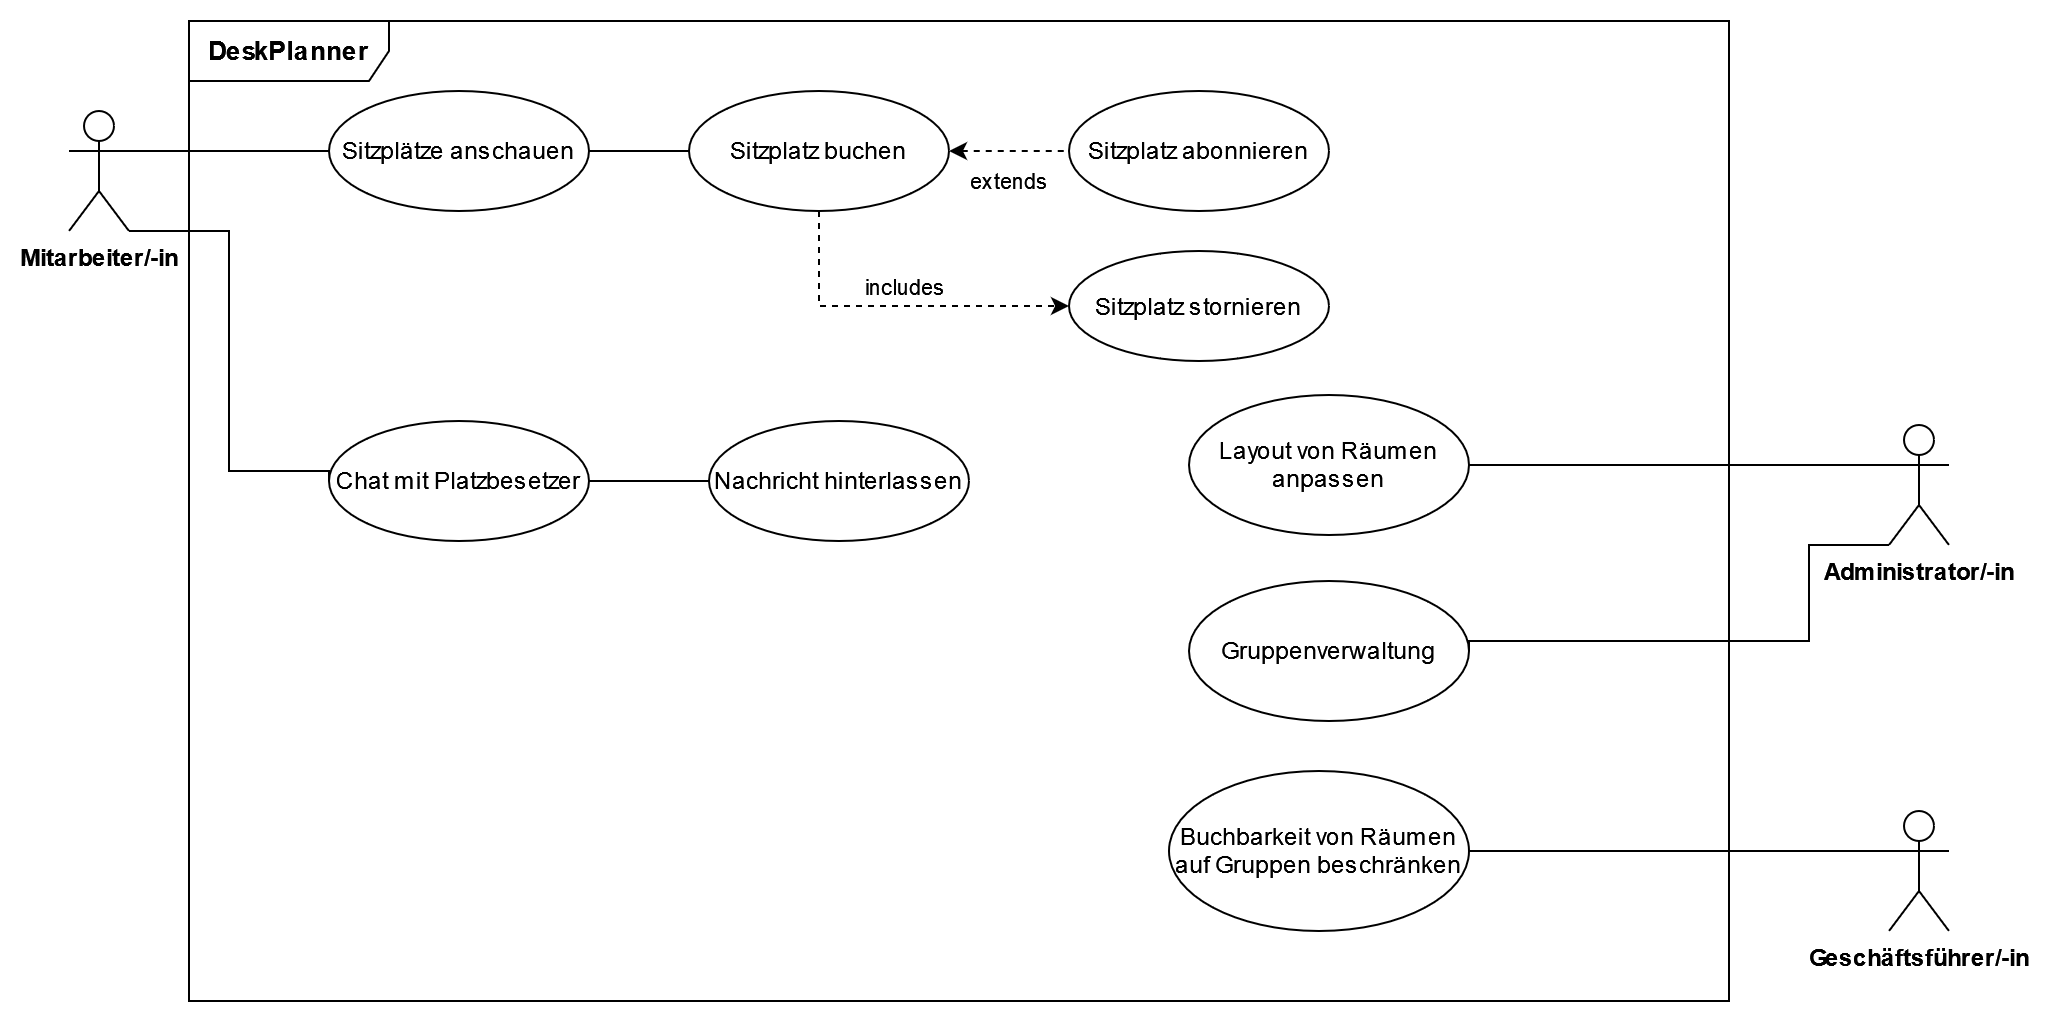
\includegraphics[width=0.8\textwidth]{UseCase_Diagram.png}
    \caption{Usecase-Diagramm}
    \label{fig:Usecase-Diagramm}
\end{figure}


\section{User Interface Entwürfe}

\section{Technisches Konzept}

\subsection{Verwendete Frameworks}

\subsection{Softwarearchitektur}

\subsection{Datenbanken}

% Bibliography
% \bibliography{file.bibtex}
\bibliographystyle{plain}

% Ending of document
\end{document}
